\section{Технический проект}
\subsection{Общая характеристика организации решения задачи}

Необходимо спроектировать и разработать веб-приложение для организации общения пользователей в чат-комнатах.

Центральным компонентом данного веб-приложения выступает серверная часть, которая играет критически важную роль в общей архитектуре. Серверная часть отвечает за предоставление набора конечных точек (endpoints), к которым могут обращаться клиентские приложения для получения необходимых данных. Эти конечные точки представляют собой интерфейсы, через которые клиентские приложения могут взаимодействовать с сервером, запрашивая и отправляя информацию. Такой подход к организации серверной части позволяет обеспечить высокую гибкость и масштабируемость системы.

Одним из ключевых преимуществ использования конечных точек является возможность создания клиентских частей для различных платформ и с использованием различных технологий. Клиентские приложения могут быть разработаны для веб-браузеров, мобильных устройств, настольных компьютеров и других платформ, и все они смогут взаимодействовать с серверной частью через стандартные конечные точки. Это означает, что разработчики могут выбирать те технологии и инструменты, которые наиболее подходят для конкретной платформы, будь то React для веб-приложений, Swift для iOS-приложений или Kotlin для Android-приложений.

Благодаря такому подходу, веб-приложение для общения пользователей в чат-комнатах может быть легко адаптировано и расширено для поддержки новых платформ и устройств по мере необходимости. Кроме того, это позволяет улучшить пользовательский опыт, так как каждое клиентское приложение может быть оптимизировано для своей платформы, обеспечивая максимальную производительность и удобство использования.

\subsection{Обоснование выбора технологии проектирования}

В разработке современных веб-приложений ключевую роль играют выбранные технологии, определяющие функциональность, производительность и удобство использования приложения. В данном разделе обосновывается выбор конкретных технологий для создания веб-приложения, которое является объектом исследования и основной темой дипломной работы.

Критерии выбора технологий включают в себя уровень поддержки, масштабируемость, безопасность, эффективность разработки и управления проектом, а также соответствие требованиям и целям приложения. В рамках исследования проводится анализ различных технологических стеков, исследуются их преимущества и недостатки с учетом специфики проекта.

Выбранные технологии должны обеспечивать возможность создания современного, отзывчивого и функционального веб-приложения, способного эффективно решать поставленные перед ним задачи и соответствовать требованиям пользователей. Обоснование выбора технологий позволит обосновать архитектурные и технические решения, принятые в рамках разработки веб-приложения, и обеспечить успешную реализацию проекта.

\subsubsection{Язык программирования C\#}

Язык программирования C\# (C Sharp) – это современный объектно-ориентированный язык программирования, разработанный корпорацией Microsoft\cite{csdocs}. Он представляет собой высокоуровневый язык с сильной статической типизацией, что означает, что типы всех данных в программе известны на этапе компиляции. Это помогает выявлять ошибки на ранних стадиях разработки и улучшает качество и безопасность кода. C\# используется для создания различных типов приложений, включая настольные, мобильные и веб-приложения. Язык тесно интегрирован с платформой .NET, которая предоставляет разработчикам широкий набор библиотек и инструментов для построения надежных и эффективных приложений.

C\# получил широкое распространение в веб-разработке благодаря фреймворку ASP.NET Core. ASP.NET Core - это кроссплатформенный фреймворк для создания веб-приложений, разработанный компанией Microsoft. Он является модернизированной и улучшенной версией платформы ASP.NET, предназначенной для создания современных, быстрых и масштабируемых веб-приложений. Одним из ключевых преимуществ ASP.NET Core является его кроссплатформенность: разработчики могут создавать и запускать приложения на различных операционных системах, включая Windows, Linux и macOS. Это делает фреймворк гибким и универсальным инструментом для разработки веб-приложений в самых разных средах.

ASP.NET Core предоставляет разработчикам широкий набор инструментов и функций, которые упрощают процесс разработки и ускоряют создание приложений. В состав ASP.NET Core включены такие технологии, как ASP.NET Core MVC, Razor Pages, ASP.NET Core Web API, ASP.NET Core Identity, SignalR и некоторые другие\cite{aspnetdocs}.

\subsubsection{Язык программирования JavaScript}

JavaScript – это интерпретируемый язык программирования высокого уровня с слабой динамической типизацией, что означает, что типы переменных определяются во время выполнения программы, а не на этапе компиляции. Этот язык поддерживается подавляющим большинством современных браузеров, благодаря чему он стал фактически стандартом для написания динамических веб-страниц. JavaScript позволяет разработчикам создавать интерактивные и динамичные элементы на веб-страницах, такие как анимации, формы, игры и многие другие компоненты, которые улучшают пользовательский опыт.

На базе JavaScript реализовано множество различных библиотек и фреймворков, которые облегчают разработку веб-приложений и расширяют функциональные возможности языка. Среди самых популярных и широко используемых библиотек и фреймворков можно выделить React, Vue, Angular и Next.js. Эти инструменты помогают разработчикам создавать масштабируемые и высокопроизводительные веб-приложения, предлагая структурированные подходы к разработке, управление состоянием, маршрутизацию, взаимодействие с сервером и многое другое.

Для реализации клиентской части нашего проекта был выбран фреймворк Next.js. Next.js – это мощный фреймворк для разработки универсальных React-приложений. Он предоставляет разработчикам набор инструментов и функциональности, которые значительно упрощают процесс разработки веб-приложений. Одной из ключевых особенностей Next.js является поддержка серверного рендеринга, что позволяет рендерить страницы на сервере перед их отправкой на клиент. Это улучшает производительность и SEO, так как страницы загружаются быстрее и поисковые системы могут их легче индексировать.

Помимо серверного рендеринга, Next.js также поддерживает статическую генерацию страниц, что позволяет создавать статические HTML-файлы на этапе сборки приложения. Эти файлы могут быть развернуты на любом веб-сервере и предоставлять мгновенную загрузку и высокую производительность. Динамический рендеринг – ещё одна мощная возможность Next.js, которая позволяет создавать страницы на лету, в зависимости от данных, предоставляемых клиентом или сервером.

Next.js также предлагает удобное управление маршрутизацией, что делает процесс навигации в приложении простым и интуитивно понятным. В отличие от некоторых других фреймворков, маршрутизация в Next.js базируется на файловой системе, что означает, что структура папок и файлов в проекте определяет маршруты приложения. Это упрощает настройку и поддержку маршрутизации, особенно в крупных проектах.

\subsubsection{JSON Web Token}

Для обеспечения авутентификации и авторизации пользователей в программной системе используется технология JSON Web Tokens (JWT).

JWT (JSON Web Token) — это открытый стандарт (RFC 7519) для создания токенов, используемых для передачи информации между участниками. Токены формируются в виде компактного, URL-безопасного JSON-объекта, который может быть подписан с помощью алгоритма HMAC или асимметричной криптографии (например, RSA). JWT состоит из трех частей: заголовка (header), полезной нагрузки (payload) и подписи (signature). Заголовок определяет тип токена и алгоритм шифрования, полезная нагрузка содержит утверждения (claims), такие как идентификация пользователя или срок действия токена, а подпись обеспечивает целостность и подлинность токена. Основное применение JWT — аутентификация и авторизация в веб-приложениях, где токены используются для передачи проверенных данных между клиентом и сервером, обеспечивая безопасный и эффективный способ управления доступом к ресурсам.


\subsection{Проектирование архитекуры программной систмеы}

\subsubsection{Компоненты разрабатываемой системы}

На рисунке \ref{components:image} в виде UML-диаграммы показана архитектура программной системы.

Данная диаграмма моделирует высокоуровневую структуру системы, отображая компоненты и их взаимосвязи. Основная цель диаграммы компонентов заключается в представлении физических и логических элементов системы, таких как модули, библиотеки, файлы и их зависимости. Компоненты являются основными строительными блоками, которые могут быть развернуты на различных узлах и взаимодействуют друг с другом через интерфейсы. Каждый компонент может включать в себя другие компоненты или быть связан с ними через четко определенные интерфейсы, что позволяет понять, как части системы работают вместе\cite{uml}.

Диаграмма компонентов используется для визуализации архитектуры системы и помогает определить и спланировать разбиение системы на автономные и заменяемые части. Это особенно полезно на этапах проектирования и разработки, когда важно понять, как отдельные части системы будут взаимодействовать друг с другом.

\begin{figure}[H]
\center{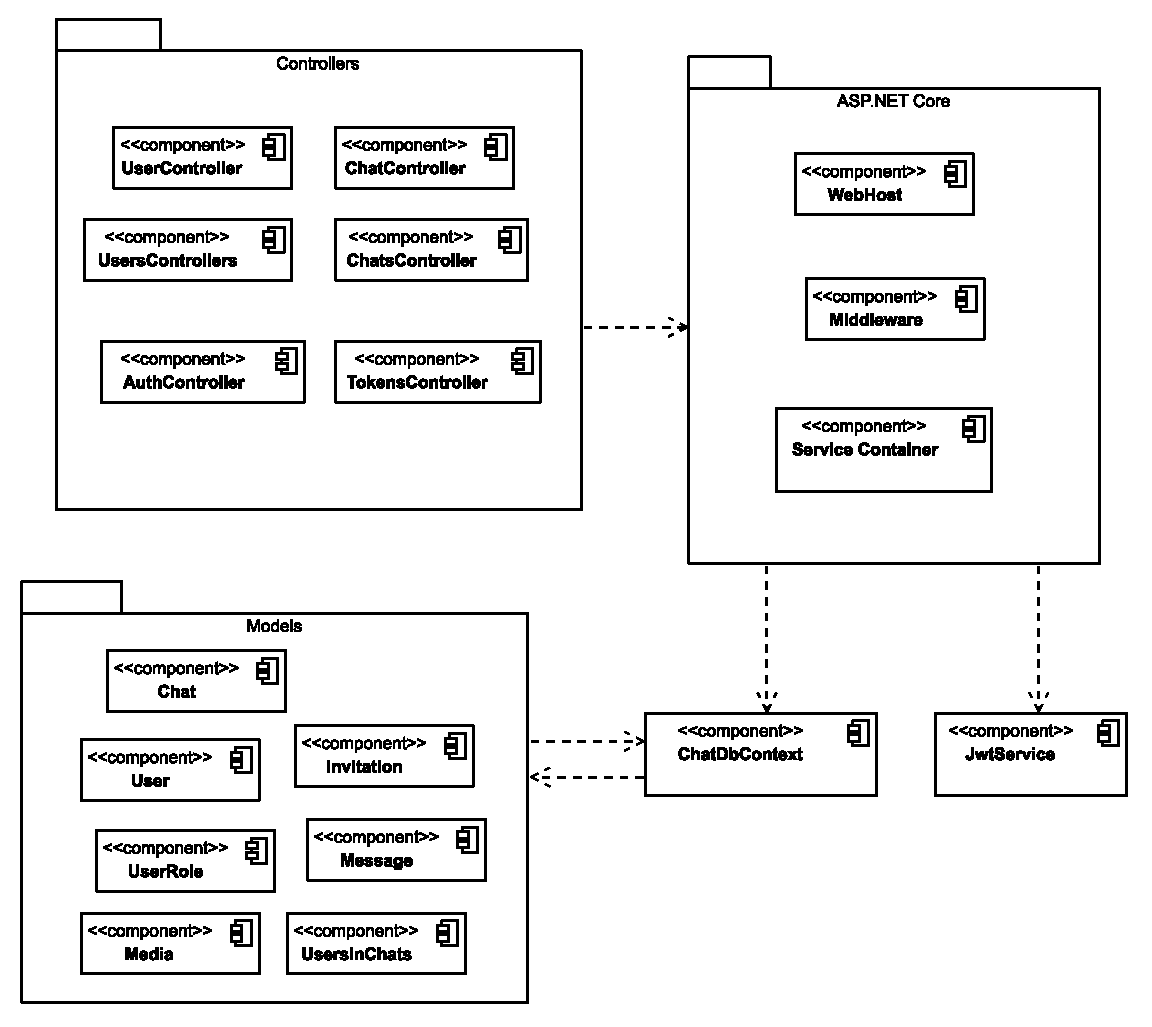
\includegraphics[width=1\linewidth]{components}}
\caption{Диаграмма компонентов}
\label{components:image}
\end{figure}

Программная система включает в себя:
\begin{enumerate}
		\item Клиентская часть: это веб-приложение, разработанное с использованием React-фреймворка Next.js. Она предоставляет пользовательский интерфейс для взаимодействия с приложением чата. Клиентская часть отображает данные, отправленные и полученные от сервера, и обрабатывает пользовательские действия, такие как отправка сообщений и управление чатами.
			
		\item Сервис авторизации: это компонент, ответственный за регистрацию пользователей и управление процессами авторизации и аутентификации в приложении. 
		
		\item Основное приложение: это серверная часть приложения, на котором работает чат. Она обрабатывает запросы от клиентской части, обеспечивает функциональность чата, такую как отправка и получение сообщений, управление пользователями и чатами, и поддерживает взаимодействие с базой данных.
		
		\item База данных: это сервер, на котором развернута PostgreSQL, отвечающая за хранение и управление данными приложения. PostgreSQL используется для хранения пользовательских аккаунтов, сообщений чата, информации о чатах и других необходимых данных. Он обеспечивает надежное хранение и управление данными, а также поддерживает выполнение сложных запросов и транзакций\cite{db}.
\end{enumerate}

\subsection{Модель данных}

На рисунке \ref{data_model:image} в виде UML-диаграммы классов представлена модель данных приложения.

Данный вид диаграмм моделирует статическую структуру системы, отображая классы, их свойства, методы и взаимоотношения между ними. Основная цель диаграммы классов заключается в представлении основных элементов системы и их взаимосвязей, что помогает разработчикам понять структуру и логику системы. Классы представлены в виде прямоугольников, разделенных на три секции: верхняя содержит имя класса, средняя – атрибуты (свойства), а нижняя – операции (методы).

Связи между классами показываются с помощью линий, которые могут быть аннотированы, чтобы указать тип отношения, например ассоциацию, агрегацию, композицию или наследование. Ассоциации показывают базовые связи между классами, агрегации указывают на отношения "часть-целое", композиции – на более сильные связи, где компоненты не могут существовать без целого, а наследование показывает иерархические отношения между классами, где один класс является расширением другого.

Диаграмма классов помогает в проектировании и документировании объектно-ориентированных систем, обеспечивая четкое представление о том, какие классы существуют в системе, какие атрибуты и методы они имеют, и как они взаимодействуют друг с другом.

\begin{landscape}
	\begin{figure}[ht]
		\center{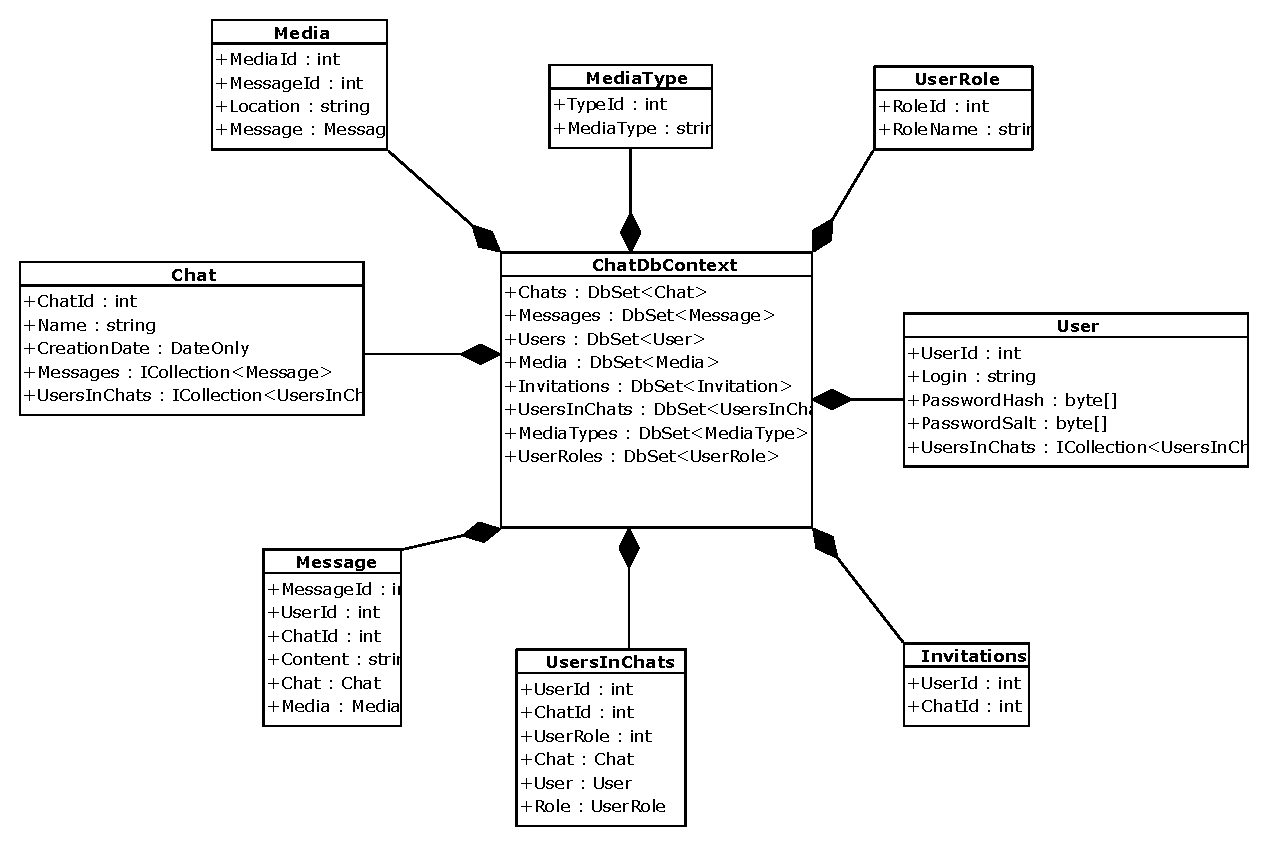
\includegraphics[scale=1.10]{data_model}}
		\caption{Диаграмма классов модели данных}
		\label{data_model:image}
	\end{figure}
\end{landscape}

\begin{itemize}
	\item ChatDbContext - класс, обеспечивающий связь моделей и БД чс Entity Framework. Также описывает правила созания объеков моделей из таблиц БД;
	\item Chat - модель, представляющая собой отображение данных чата;
	\item Media - модель, представляющая собой отображение медиа-файла;
	\item MediaType - модель, представляющая собой отображение типа медиа-файла;
	\item Invitation - модель, представляющая собой отображение приглашения в чат;
	\item Message - модель, представляющая собой отображение данных сообщения;
	\item User - модель, представляющая собой отображение данных пользователя;
	\item UserRole - модель, представляющая собой отображение данных типа роли пользователя;
	\item UsersInChats - модель, представляющая собой отображение данных связи пользователей с их чатами.
\end{itemize}

\subsection{Контроллеры}

На рисунке \ref{controllers:image} представлена диаграмма классов-контроллеров и сервисов, необходимых для их работы.

\begin{landscape}
	\begin{figure}[ht]
		\center{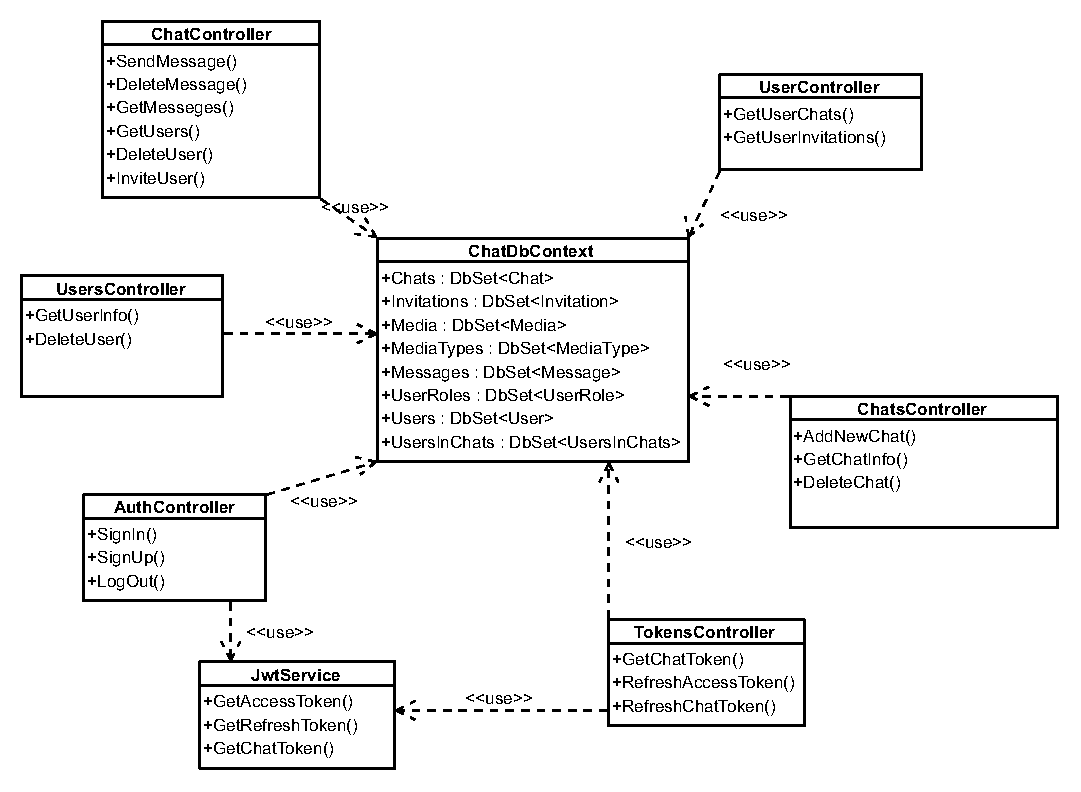
\includegraphics[scale=1.10]{cd_controllers}}
		\caption{Диаграмма классов-контроллеров}
		\label{controllers:image}
	\end{figure}
\end{landscape}

Спецификация диаграммы классов-контроллеров:
\begin{itemize}
	\item ChatDbContext - класс, обеспечивающий связь моделей приложения с фреймворком Entity Framework и предоставляющий доступ контроллерам к данным БД\cite{ef};
	\item JwtService.cs - класс, предоставляющий методы работы с JWT-токенами;
	\item ChatController.cs - класс, предосталяющий методы для работы с конкретным чатом;
	\item UserController.cs - класс, предоставляющий методы для работы с конкретным пользователем приложения;
	\item ChatsController.cs - класс, предоставляющий методы для работы со всеми чатами;
	\item UsersController.cs - класс, предоставляющий методы для работы со всеми пользователями приложения;
	\item AuthController.cs - класс, предоставляющий методы для аутентификации и регистрации пользователей приложения;
	\item TokensController.cs - класс, предоставляющий методы для полуения и обновления токенов.
\end{itemize}

\subsubsection{Представления}

В фреймворке Next.js структура приложения представлена набором страниц, которые в свою очередь состоят из React-компонентов. Компоненты React представляют собой совокупность HTML-подобной разметки и кода JavaScript (TypeScript) для управления состоянием компонента и загрузкой необходимых для отображения данных\cite{nextjs}.

Разрабатываемое прилложение будет содержать следующие страницы:
\begin{itemize}
	\item signup.tsx является представлением для регистрации в приложении;
	\item signin.tsx является представлением для входа в приложение;
	\item main.tsx (включает в себя комоненты AppNavigation, ChatMenu, ChatRoom, Messages, Modal) является основным представлением приложения. Отображает навигацию по приложению и сам чат;
	\item user.tsx представление личного кабинета пользователя для управления персональными данными.
\end{itemize}

\subsubsection{Маршруты приложения}

Для обеспечения доступа пользователей к необходимым информационным ресурсам приложения, разработана карта маршрутов приложения. Описание маршрутов приведено ниже.

POST /Auth/signup - маршрут, предназначенный для регистрации пользователей в приложении. В теле запроса принимает логин и пароль регистрируемого пользователя.

POST /Auth/signin - маршрут, предназначенный для входа пользователей в приложении. В теле запроса принимает логин и пароль пользователя.

GET /Tokens/chat-token - маршрут, предназначенный для выдачи токенов чатов.

GET /Tokens/refresh-chat-token - маршрут, предназначенный для обновления токенов чатов.

GET /Tokens/refresh-access-token - маршрут, предназначенный для обновления токенов доступа.

POST /Chat/send-message - маршрут, предназначенный для отправки сообщений в чате. В теле запроса принимает текст сообщения.

DELETE /Chat/delete-message - маршрут, предназначенный для удаления сообщений из чата. В теле запроса принимает идентификатор удаляемого сообщения.

GET /Chat/messages - маршрут, предназначенный для получения сообщений чата.

GET /Chat/users - маршрут, предназначенный для получения пользователей чата.

POST /Chat/invite - маршрут, предназначенный для приглашения новых пользователей в чат.

DELETE /Chat/delete-user - маршрут, предназначенный для удаления пользователей из чата. В теле запроса принимает идентификатор удаляемого пользователя.

POST /Chats - маршрут, предназначенный для создания нового чата. В теле запроса принимает информацию для создания нового чата.

DELETE /Chats - маршрут, предназначанный для удаления чата. В теле запроса принимает идентификатор удаляемого чата.

GET /User/chats - маршрут, предназначенный для получения чатов, в которых состоит пользователь.

GET /User/invitations - маршрут, предназначенный для получения приглашений пользователя в чаты.

GET /Users - маршрут, предназначенный для полученя информации о конкретном пользователе. В теле запроса принимает идентификатор пользователя, информацию о котором необходимо получить.

DELETE /Users - маршрут, предназначенный для удаления пользователя. В теле запроса принимает идентификатор удаляемого пользователя.

На рисунке \ref{routes:image} представлена схема маршрутов приложения.

\begin{landscape}
	\begin{figure}[ht]
		\center{\includegraphics[width=1\linewidth]{routes}}
		\caption{Маршруты приложения}
		\label{routes:image}
	\end{figure}
\end{landscape}

\subsubsection{Проект данных разрабатываемой системы}

Для организации данных, используемых в разрабатываемой системе, была выбрана реляционная БД PostgreSQL. 

PostgreSQL — это объектно-реляционная система управления базами данных с открытым исходным кодом. Она отличается высокой производительностью, надежностью и масштабируемостью. PostgreSQL поддерживает стандарт SQL и предлагает множество дополнительных возможностей, таких как полнотекстовый поиск, индексирование, транзакции с поддержкой ACID, расширения для различных типов данных, включая JSON и XML. Система активно развивается и поддерживается сообществом, что обеспечивает её актуальность и адаптацию к современным требованиям. PostgreSQL подходит для различных типов приложений, от небольших веб-приложений до крупных корпоративных систем.

Был выбран подход Database First\cite{ef}, т. е. сначала разрабатывается схема БД, а затем на ее основе средствами Entity Framework генерируются модели приложения.

Схема БД состоит из следующих таблиц:
\begin{itemize}
	\item chats - чаты;
	\item invitations - приглашения пользователей в чаты;
	\item messages - сообщения в чатах;
	\item media - загруженные файлы;
	\item media\_type - тип загруженного файла;
	\item user - пользователи приложения;
	\item user\_role - роли пользователей;
	\item users\_in\_chats - таблица связи пользователей и чатов, в которых они состоят. 
\end{itemize}

ER-диаграмма БД представлена на рисунке \ref{erd:image}.

\begin{figure}[H]
	\center{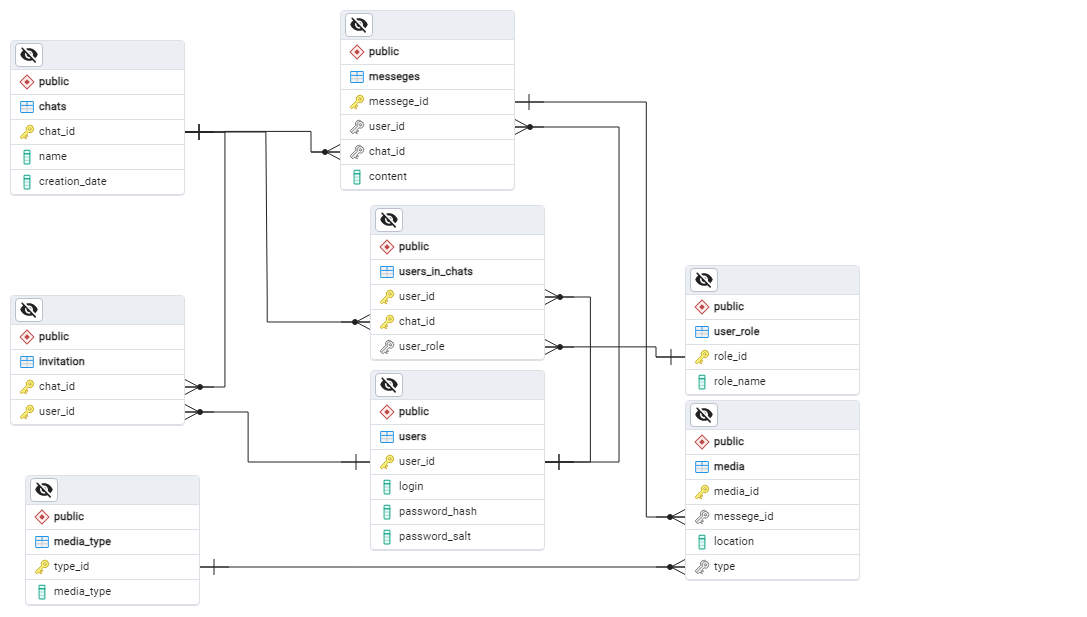
\includegraphics[width=1\linewidth]{erd}}
	\caption{ER-диаграмма базы данных}
	\label{erd:image}
\end{figure}

В таблице \ref{chats:table} представлены атрибуты сущности "<Чат">.

\begin{xltabular}{\textwidth}{|X|p{2.5cm}|p{3cm}|>{\setlength{\baselineskip}{0.7\baselineskip}}p{4.83cm}|}
	\caption{Описание полей таблицы "chats"\label{chats:table}} \hline
	\centrow Поле & \centrow Тип & \centrow Обязательное & \centrow Описание \\ \hline
	\centrow 1 & \centrow 2 & \centrow 3 & \centrow 4\\ \hline
	\endfirsthead
	\continuecaption{Продолжение таблицы \ref{chats:table}} \hline
	\centrow 1 & \centrow 2 & \centrow 3 & \centrow 4\\ \hline
	\finishhead
	chat\_id & integer & да & Идентификатор чата (автоматический) \\ \hline
	name & character varying(128) & да & Название чата \\ \hline
	creation\_date & date & да & Дата создания чата \\ \hline
\end{xltabular}

В таблице \ref{invitations:table} представлены атрибуты сущности "<Приглашение">.

\begin{xltabular}{\textwidth}{|X|p{2.5cm}|p{3cm}|>{\setlength{\baselineskip}{0.7\baselineskip}}p{4.83cm}|}
	\caption{Описание полей таблицы "invitations"\label{invitations:table}} \hline
	\centrow Поле & \centrow Тип &  \centrow Обязательное & \centrow Описание \\ \hline
	\centrow 1 & \centrow 2 & \centrow 3 & \centrow 4\\ \hline
	\endfirsthead
	\continuecaption{Продолжение таблицы \ref{invitations:table}} \centrow 1 & \centrow 2 & \centrow 3 & \centrow 4\\ \hline
	\finishhead
	chat\_id & integer & да & Идентификатор чата \\ \hline
	user\_id & integer & да & Идентификатор приглашемого пользователя \\ \hline
\end{xltabular}

В таблице \ref{messages:table} представлены атрибуты сущности "<Сообщение">.

\begin{xltabular}{\textwidth}{|X|p{2.5cm}|p{3cm}|>{\setlength{\baselineskip}{0.7\baselineskip}}p{4.83cm}|}
	\caption{Описание полей таблицы "messages"\label{messages:table}} \hline
	Поле & Тип & Обязательное & Описание \\ \hline
	\centrow 1 & \centrow 2 & \centrow 3 & \centrow 4\\ \hline
	\endfirsthead
	\continuecaption{Продолжение таблицы \ref{messages:table}} \hline
	\centrow 1 & \centrow 2 & \centrow 3 & \centrow 4\\ \hline
	\finishhead
	message\_id & integer & да & Идентификатор сообщения (автоматический) \\ \hline
	user\_id & integer & нет & Идентификатор пользователя (если есть) \\ \hline
	chat\_id & integer & да & Идентификатор чата \\ \hline
	content & text & нет & Содержание сообщения \\ \hline
\end{xltabular}

В таблице \ref{media:table} представлены атрибуты сущности "<Медиа">.

\begin{xltabular}{\textwidth}{|X|p{2.5cm}|p{3cm}|>{\setlength{\baselineskip}{0.7\baselineskip}}p{4.83cm}|}
	\caption{Описание полей таблицы "media"\label{media:table}} \hline
	Поле & Тип & Обязательное & Описание \\ \hline
	\centrow 1 & \centrow 2 & \centrow 3 & \centrow 4\\ \hline
	\endfirsthead
	\continuecaption{Продолжение таблицы \ref{media:table}} \hline
	\centrow 1 & \centrow 2 & \centrow 3 & \centrow 4\\ \hline
	\finishhead
	media\_id & serial & да & Идентификатор медиа (автоматический) \\ \hline
	location & text & да & Местоположение медиа \\ \hline
	type & integer & да & Тип медиа \\ \hline
\end{xltabular}

В таблице \ref{media_type:table} представлены атрибуты сущности "<Тип медиа">.

\begin{xltabular}{\textwidth}{|X|p{2.5cm}|p{3cm}|>{\setlength{\baselineskip}{0.7\baselineskip}}p{4.83cm}|}
	\caption{Описание полей таблицы "media\_type"\label{media_type:table}} \hline
	\centrow Поле & \centrow Тип & \centrow Обязательное & \centrow Описание \\ \hline
	\centrow 1 & \centrow 2 & \centrow 3 & \centrow 4\\ \hline
	\endfirsthead
	\continuecaption{Продолжение таблицы \ref{media_type:table}} \centrow 1 & \centrow 2 & \centrow 3 & \centrow 4\\ \hline
	\finishhead
	type\_id & int & да & Идентификатор типа медиа \\ \hline
	media\_type & character varying(20) & да & Тип медиа \\ \hline
\end{xltabular}

В таблице \ref{users:table} представлены атрибуты сущности "<Пользователь">.

\begin{xltabular}{\textwidth}{|X|p{2.5cm}|p{3cm}|>{\setlength{\baselineskip}{0.7\baselineskip}}p{4.83cm}|}
	\caption{Описание полей таблицы "users"\label{users:table}} \hline
	\centrow Поле & \centrow Тип & \centrow Обязательное & \centrow Описание \\ \hline
	\centrow 1 & \centrow 2 & \centrow 3 & \centrow 4\\ \hline
	\endfirsthead
	\continuecaption{Продолжение таблицы \ref{users:table}} \hline
	\centrow 1 & \centrow 2 & \centrow 3 & \centrow 4\\ \hline
	\finishhead
	user\_id & integer & да & Идентификатор пользователя (автоматический) \\ \hline
	login & character varying(64) & да & Логин пользователя \\ \hline
	password\_hash & bytea & да & Хэш пароля пользователя \\ \hline
	password\_salt & bytea & да & Соль пароля пользователя \\ \hline
\end{xltabular}

В таблице \ref{user_role:table} представлены атрибуты сущности "<Роль пользователя">.

\begin{xltabular}{\textwidth}{|X|p{2.5cm}|p{3cm}|>{\setlength{\baselineskip}{0.7\baselineskip}}p{4.83cm}|}
	\caption{Описание полей таблицы "user\_role"\label{user_role:table}} \hline
	\centrow Поле & \centrow Тип & \centrow Обязательное & \centrow Описание \\ \hline
	\centrow 1 & \centrow 2 & \centrow 3 & \centrow 4\\ \hline
	\endfirsthead
	\continuecaption{Продолжение таблицы \ref{user_role:table}} \\ \hline
	\centrow 1 & \centrow 2 & \centrow 3 & \centrow 4\\ \hline
	\finishhead
	role\_id & integer & да & Идентификатор роли пользователя \\ \hline
	role\_name & character varying(15) & да & Наименование роли пользователя \\ \hline
\end{xltabular}

В таблице \ref{users_in_chats:table} представлены атрибуты сущности "<Пользователи в чатах">.

\begin{xltabular}{\textwidth}{|X|p{2.5cm}|p{3cm}|>{\setlength{\baselineskip}{0.7\baselineskip}}p{4.83cm}|}
	\caption{Описание полей таблицы "users\_in\_chats"\label{users_in_chats:table}} \hline
	\centrow Поле & \centrow Тип & \centrow Обязательное & \centrow Описание \\ \hline
	\centrow 1 & \centrow 2 & \centrow 3 & \centrow 4\\ \hline
	\endfirsthead
	\continuecaption{Продолжение таблицы \ref{users_in_chats:table}} \hline \centrow 1 & \centrow 2 & \centrow 3 & \centrow 4\\ \hline
	\endhead
	Поле & Тип & Обязательное & Описание \\ \hline
	\finishhead
	user\_id & integer & да & Идентификатор пользователя \\ \hline
	chat\_id & integer & да & Идентификатор чата \\ \hline
	user\_role & integer & да & Роль пользователя в чате \\ \hline
\end{xltabular}

\subsection{Проектирование пользоватеьского интерфейса}

Учитывая требования к пользовательскому интерфейсу, сформированные в пункте технического задания, был разработан интерфейс программной системы. 

Ниже приведены макеты интерфейса десктопной версии приложения. В мобильной версии компоненты такие же как и в десктопной, но размещены с учетом удобства использования на портативных устройствах.

На рисунках ниже компоненты интерфейса пронумированы.

На рисунке \ref{signup_maket:image} представлен макет страницы регистрации. Эта страница содержит следующие компоненты:
\begin{itemize}
	\item поле для ввода логина;
	\item поле для ввода пароля;
	\item поле для ввода подтверждения пароля;
	\item кнопка "<Зарегистрироваться">;
	\item кнопка "<Войти">.
\end{itemize}

\begin{figure}[H]
	\center{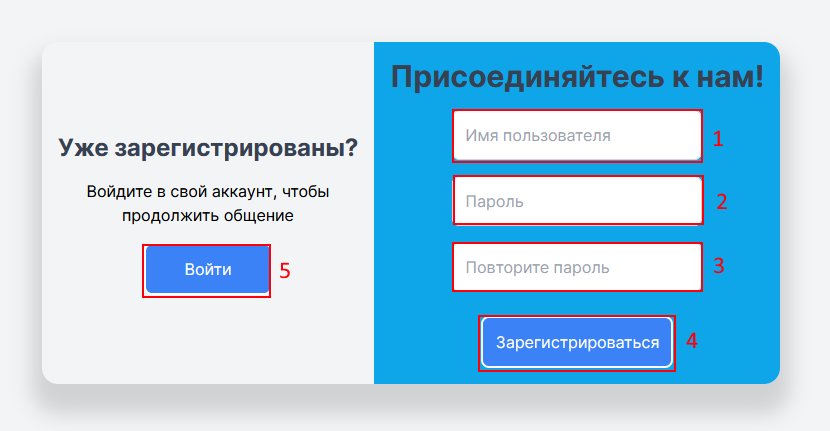
\includegraphics[width=1\linewidth]{signup_maket}}
	\caption{Макет страницы регистрации}
	\label{signup_maket:image}
\end{figure}

На рисунке \ref{signin_maket:image} представлен макет страницы входа. Эта страница содержит следующие компоненты:
\begin{itemize}
	\item поле для ввода логина;
	\item поле для ввода пароля;
	\item кнопка "<Войти">;
	\item сссылка на страницу регистрации.
\end{itemize}

\begin{figure}[H]
	\center{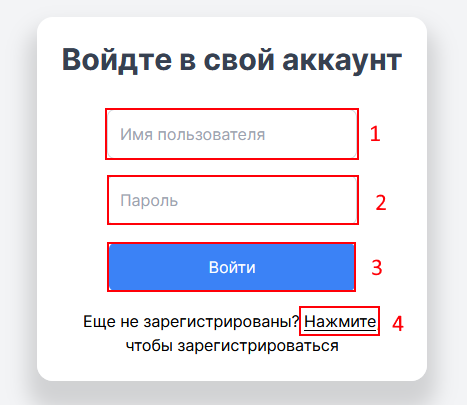
\includegraphics[width=1\linewidth]{signin_maket}}
	\caption{Макет страницы входа}
	\label{signin_maket:image}
\end{figure}

На рисунке \ref{main_maket:image} представлен макет страницы входа. Эта страница содержит следующие компоненты:
\begin{itemize}
	\item список чатов;
	\item кнопка перехода на страницу пользователя;
	\item кнопка создания чата;
	\item кнопка поиска по чатам;
	\item вкладка "<Чаты">;
	\item вкладка "<Приглашения">;
	\item список сообщений чата;
	\item кнопка меню настроек чата;
	\item кнопка отпраки файла;
	\item поле ввода сообщения;
	\item кнопка отправки сообщения.
\end{itemize}

\begin{figure}[H]
	\center{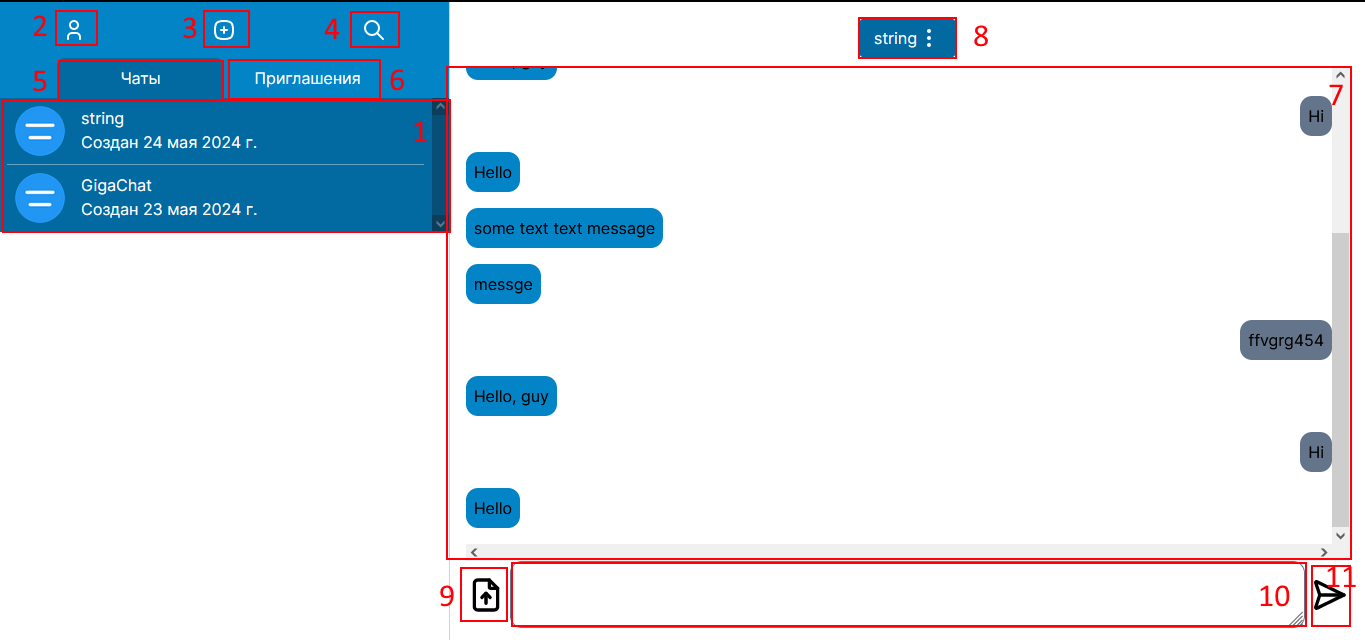
\includegraphics[width=1\linewidth]{main_maket}}
	\caption{Макет основной страницы}
	\label{main_maket:image}
\end{figure}

На рисунке \ref{cabinet_maket:image} представлен макет страницы входа. Эта страница содержит следующие компоненты:
\begin{itemize}
	\item поле для изменения логина пользователя;
	\item кнопка для подтверждения изменения логина;
	\item поле для изменения пароля пользователя;
	\item поле для подтверждения нового пароля;
	\item кнопка для подтверждения изменения пароля.
\end{itemize}

\begin{figure}[H]
	\center{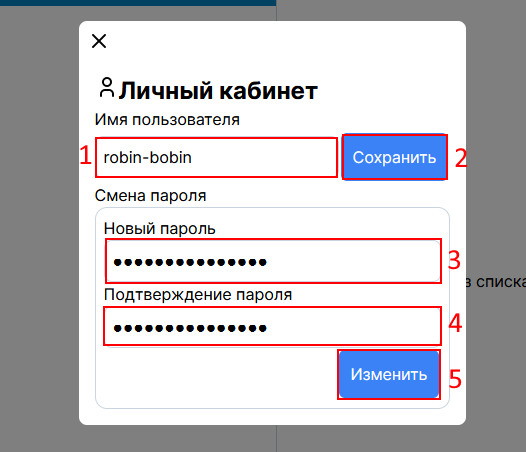
\includegraphics[width=1\linewidth]{cabinet_maket}}
	\caption{Макет кабинет пользователя}
	\label{cabinet_maket:image}
\end{figure}